% -*- mode: latex; coding: utf-8 -*-
% $Id: article.tex 739 2009-06-18 12:29:54Z elric $

\documentclass[times, 10pt,twocolumn]{article}
\usepackage{amssymb,amsmath,amsthm,amscd,bm}

\usepackage{listings}
\lstset{language=C++, basicstyle=\normalsize}

\usepackage{graphicx}

\usepackage[normalsize]{subfigure}

%\usepackage{algorithm}
%\usepackage{algorithmic}
\usepackage[named]{algo}

\usepackage{ieee}
\usepackage{times}
\usepackage{expdlist}

\newcommand{\gC}{\mathfrak{C}}
\newcommand{\gD}{\mathfrak{D}}
\newcommand{\gF}{\mathfrak{F}}
\newcommand{\gG}{\mathfrak{G}}
\newcommand{\gH}{\mathfrak{H}}
\newcommand{\gK}{\mathfrak{K}}
\newcommand{\gR}{\mathfrak{R}}
\newcommand{\gN}{\mathfrak{N}}
\newcommand{\gP}{\mathfrak{P}}
\newcommand{\gf}{\mathfrak{f}}

\newcommand{\cR}{\mathcal{R}}

\newcommand{\nT}{\mathbb{T}}
\newcommand{\Nat}{\mathbb{N}}

\newcommand{\gFs}{\gF^*}
\newcommand{\gFu}{\gF^{\cup}}

\newcommand{\executes}{\textit{executes}}
\newcommand{\pure}{\textit{pure}}
\newcommand{\params}{\textit{params}}
\newcommand{\func}{\textit{func}}
\newcommand{\adj}{\textit{adj}}
\newcommand{\any}{\textit{any}}
\newcommand{\isPrim}{\textit{isPrimitive}}
\newcommand{\isSol}{\textit{isSolution}}
\newcommand{\isPartSol}{\textit{isPartSolution}}
\newcommand{\fixed}{\textit{fixed}}
\newcommand{\children}{\textit{children}}
\newcommand{\type}{\textit{type}}
\newcommand{\merge}{\textit{merge}}
\newcommand{\vtable}{\textit{vtable}}
\newcommand{\adjacent}{\textit{adjacent}}
\newcommand{\parents}{\textit{parents}}

\newcommand{\nlhd}{\ntriangleleft}
\newcommand{\nrhd}{\ntriangleright}

\newtheorem{statement}{Statement}
\newtheorem{lemma}{Lemma}
\newtheorem{theorem}{Theorem}


%\pagestyle{empty} !!!!

\pagestyle{plain}

\begin{document}

\title{Reconstruction of Class Hierarchies for Decompilation of C++ Programs}

\author{A. Fokin\\
Moscow State University\\
Computational Math. and Cybernetics Dept.\\
Leninskie Gory, Moscow, Russia\\
apfokin@gmail.com
\and
K. Troshina\\
Institute for System Programming\\
Russian Academy of Sciences\\
25, Alexander Solzhenitsyn st., Moscow, Russia\\
katerina@ispras.ru
\and
A. Chernov\\
Moscow State University\\
Computational Math. and Cybernetics Dept.\\
Leninskie Gory, Moscow, Russia\\
cher@unicorn.cmc.msu.ru
}

\maketitle
\thispagestyle{empty}

\begin{abstract}
This paper presents a method for automatic reconstruction of
polymorphic class hierarchies from assembly code obtained by
compiling a C++ program. If the program was compiled with
run-time type information (RTTI), class hierarchy is
reconstructed via analysis of RTTI structures.

In case RTTI structures are missing in the assembly,
a technique based on analysis
of virtual tables and virtual destructors is used.
An inheritance relation on a set of classes induces
an inheritance relation on a set of virtual tables.
If virtual inheritance is not used,
then induced relation on a set of virtual tables
is a single inheritance relation.
The presented technique is used for reconstruction
of this single inheritance relation.
Information on virtual function tables belonging to classes
that use multiple inheritance is also gathered during reconstruction.
\end{abstract}

\section{Introduction}

Decompilation from low-level machine languages to high-level
languages (especially C) has gained fair amount of attention
recently. Decompilers have been improving in quality and range
of accepted low-level programs. The C programming languages
was chosen as the target language for decompilers essentially
because it is simple enough yet powerful and widely used.
However, a part of programs subject for decompilation were
actually written in C++ or C/C++ mix. Decompilation of C++
programs into C results in undesirable artefacts like
non-decompiled assembly fragments in place of C++ exception
handling operators, or mess of C types instead of C++
inheritance hierarchy. Therefore recovering of C++ specific
language features is important for quality decompilation.
This work is an step on this way.

%Over the last few years there has been a lot of work on
%automatic decompilation of arbitrary assembly programs into
%high-level programming languages, such as C. C programming
%language is still widely used, especially in applications that
%were being developed for over 10 years. Compared to C, C++ uses
%object-oriented approach to design and development. For a long
%time, support of C++ in compilers was incomplete, with most of
%compilers handling C++ features differently, and therefore being
%incompatible. At that time C was the only option for writing
%cross-platform code. During the last years support of C++ in
%compilers has been substantially improved, and it is frequently
%used in modern applications.

%Compared to C, C++ introduces several new concepts. In case decompilation is performed to aid understanding of the program, it is desirable to reconstruct them during decompilation. Polymorphic classes, i.e. classes that define one or several virtual functions, are one of such concepts. Hierarchy of such classes reveals the structure of the application, and simplifies understanding its principles of operation.

In this work we present a method for reconstruction of
hierarchies of polymorphic classes from assembly code obtained
by compiling a C++ program. We presume that no modifications of
the assembly code were performed after compilation (such as
assembly-level obfuscation).

If the program was compiled with run-time type information
(RTTI) enabled, hierarchy of polymorphic classes is
reconstructed
exactly as it was in the source C++ program. Multiple and
virtual inheritance are handled correctly. As run-time type
information structures store class names, class names are also
recovered.

If the program was compiled without run-time type information,
we consider an induced inheritance relation on
a set of virtual function tables.
This relation is reconstructed via analysis of virtual function
tables and virtual destructors.
Multiple inheritance is also partially handled by gathering
information on virtual function tables.

For a prototype implementation we considered C++ ABI
(application binary interface) of Microsoft Visual Studio
compiler on Windows platform and C++ ABI
of GNU C++ compiler on Windows. We use MSVC 9.1 and G++ 4.2.4
for experimental study, but the prototype tool also work for
other versions of these compilers provided they use the same C++ ABI.

The paper is organized as follows. Section
\ref{sectionRelatedWork} discusses related work.
Class hierarchy reconstruction via analysis of RTTI structures
is presented in Section \ref{sectionRTTIAnalysis}.
Section \ref{sectionNoRTTIAnalysis} presents methods for class
hierarchy reconstruction without RTTI structures.
The experimental results are discussed in Section \ref{sectionExperiments}.
Our conlusions and directions for future work are
presented in the last section.

%The rest of this paper is organized as follows. Section 2 provides a short outline of existing solutions of the problem. In section 3 the

\section{Related work}
\label{sectionRelatedWork}

There have been a relatively small amount of work
on automatic reconstruction of class hierarchies from assembly code. 

Sabanal and Yason \cite{sabanal07} have proposed
a technique based on the analysis of constructors and destructors.
In case RTTI is present,
information on class hierarchy is extracted from RTTI structures.
If RTTI is not present, classes are identified by searching for constructors,
destructors and virtual tables.
This approach also allows detecting non-polymorphic classes in some cases.
Class relationship inference for polymorphic classes is done via constructor
analysis.
%No details on implementation and handling of special cases are provided.

Skochinsky \cite{skochinsky06} has given a detailed description
of RTTI structures used by MSVC,
along with implementation details of some of the C++ concepts,
such as constructors and destructors.
He has successfully used RTTI structure analysis
for polymorphic class hierarchy reconstruction.

% maybe Emmerik?
Paper \cite{emmerik04} describes
the experience gained from applying
a native executable decompiler,
assisted by a commercial disassembler and hand editing,
to a real-world Windows-based application.
Authors were able to recover almost all original class names
and the complete class hierarchy via analysis of RTTI structures.

%\section{Class hierarchy reconstruction via analysis of RTTI structures}
\section{Analysis of RTTI structures}
\label{sectionRTTIAnalysis}

\subsection{Run-time type information in C++}
Run-time type information in C++ is used for
implementing the following operators:

\begin{itemize}
\item The \lstinline{dynamic_cast<>} operator.
This operator performs type conversions at run time.
The \lstinline{dynamic_cast<>} operator guarantees
the conversion of a pointer to a base class to a pointer to a
derived class, or the conversion of an lvalue referring
to a base class to a reference to a derived class.
A program can thereby use a class hierarchy safely.

\item \lstinline{typeid} operator. This operator provides a program with the ability to retrieve the actual type of an object referred to by a pointer or a reference.
\end{itemize}

The \lstinline{typeid} operator can be applied to non-polymorphic types.
In this case it is evaluated at compile time.
On the contrary, the \lstinline{dynamic_cast<>} operator works
with polymorphic types only, and results in undefined behavior
in case the program was compiled without RTTI.

The layout of RTTI structures used for implementing
the \lstinline{typeid} and the \lstinline{dynamic_cast<>} operators
is defined by the application binary interface (ABI) used by the C++ compiler.
The layout varies from compiler to compiler and from platform to platform.
For example, Microsoft uses an undocumented format,
which, however, has been successfully reverse-engineered,
and can be looked up in source code of Wine. \if 0 \cite{wine} \fi
The layout of RTTI structures used in GCC is defined in
the \lstinline{<cxxabi.h>} header file, which is supplied with the compiler.
In this paper we presume that the format of RTTI structures
used by the compiler is known and can be parsed.

\subsection{Class hierarchy reconstruction}

In case RTTI structures are present in assembly,
the process of class hierarchy reconstruction can be split
into the following steps:

\begin{enumerate}\compact
\item Locate RTTI structures.
\item Parse RTTI structures.
\item Use obtained information to reconstruct a polymorphic class hierarchy.
\end{enumerate}

The layout of the RTTI structures in assembly is determined
by the ABI used.
As there are quite few different RTTI layouts,
it is practical to repeat the above steps several times,
once for each layout,
and then choose the most plausible variant manually.

In certain cases it is possible to determine the compiler used.
%
% for producing the assembly. In case format of RTTI structures the compiler uses is known, steps 1-3 can be run only once.
Firstly, it can be determined by analyzing the standard library
the program uses. If the standard library is linked dynamically,
the compiler can easily be determined given the shared library file.
If the standard library is linked statically,
its vendor can be determined via function signature comparison.

Given the layout and position of the RTTI structures in assembly,
parsing them imposes no difficulties.
Then full polymorphic class hierarchy
can be reconstructed by merging all partial class hierarchies
obtained from RTTI structures.

\subsection{Locating the RTTI structures}

In all ABIs known to the moment the pointer to the RTTI structure
of a class always precedes the corresponding virtual function table,
so it can be accessed like \verb|vptr[-1]|.
Therefore, the problem of finding the RTTI structures can be reduced
to a problem of locating virtual function tables.
For each virtual function table the following statements hold:
\begin{itemize}\compact
%\item Virtual function table is stored in data segment.
\item Each virtual function table is an array of pointers to functions.
\item Only the first element of the virtual function table
is referenced from program code --- its address
is used in constructors and destructor of the corresponding class. 
\end{itemize}

Algorithm \ref{alg:find_vtables} makes use of these statements
for finding virtual function tables. It uses the following functions:

$\textit{isReferenced}$ --- determines whether the given address
is referenced from the program code.

$\textit{isPointerToFunction}$ --- determines whether the given pointer
is a pointer to a function.

\if 0
\begin{figure}[htb!]
\begin{algorithmic}[1]
\STATE $p \gets \textit{DataSegment}_{\textit{start}}$
\WHILE{$p < \textit{DataSegment}_{\textit{end}}$}
    \STATE $p' \gets p$
    \STATE $p \gets p + \text{\lstinline{sizeof(void*)}}$
    \IF{$\textit{isReferenced}(p') ~ \textbf{and} ~ \textit{isPointerToFunction}(\text{\lstinline{*}}p')$}
        \STATE $\textit{vTableSize} \gets 1$
        \LOOP
            \IF{$\textit{isReferenced}(p) ~ \text{\textbf{or not}} ~ \textit{isPointerToFunction}(\text{\lstinline{*}}p)$}
                \STATE \textbf{break}
            \ENDIF
            \STATE $\textit{vTableSize} \gets \textit{vTableSize} + 1$
            \STATE $p \gets p + \text{\lstinline{sizeof(void*)}}$
        \ENDLOOP
        \STATE \textbf{store} vtable at $p$ of size $\textit{vTableSize}$
    \ENDIF
\ENDWHILE
\end{algorithmic}
\caption{Algorithm for locating virtual function tables.}
\label{alg:find_vtables}
\end{figure}
\fi

\begin{figure}[htb!]
\small
\lstset{basicstyle=\small}
\begin{minipage}[b]{0.5\textwidth}
\begin{algorithm}{LocateVTables}{
    \label{alg:find_vtables}
    \qoutput{Set of pairs (virtual table position, virtual table size)}
}
$\textit{vTables} \gets \emptyset$ \\
$p \gets \textit{DataSegment}_{\textit{start}}$ \\
\qwhile $p < \textit{DataSegment}_{\textit{end}}$ \qdo \\
    \qif $\textit{isReferenced}(p) ~ \textbf{and} ~ \textit{isPointerToFunction}(\text{\lstinline{*}}p)$ \qthen \\
        $\textit{vTableSize} \gets 0$ \\
        $p' \gets p$ \\
        \qrepeat \\
            $p \gets p + \text{\lstinline{sizeof(void*)}}$ \\
            $\textit{vTableSize} \gets \textit{vTableSize} + 1$
        \quntil $\textit{isReferenced}(p)$ \qor \qnot $\textit{isPointerToFunction}(\text{\lstinline{*}}p)$ \\
        $\textit{vTables} \gets \textit{vTables} \cup \{(p', \textit{vTableSize})\}$ \\
    \qelse \\
        $p \gets p + \text{\lstinline{sizeof(void*)}}$ 
    \qfi
\qelihw \\
\qreturn \textit{vTables}
\end{algorithm}
\end{minipage}
\end{figure}

%\section{Class hierarchy reconstruction in case of absence of RTTI structures}
\section{Absence of RTTI structures}
\label{sectionNoRTTIAnalysis}

Run-time type information in C++ programs
is considered frequently misused \cite{stroustrup93},
and some modern applications written in C++ refrain from using it.
The virtual function tables are still generated for each polymorphic class,
however, uniqueness of virtual function tables for each class
is not guaranteed, i.e. the same virtual function table
can be shared by several different classes.

As it was stated in the introduction,
we assume that the source C++ program does not use virtual inheritance.
That means that the induced inheritance relation
on a set of virtual functions is a single inheritance relation. 

A set of all virtual function tables $\gC$
can be built using algorithm \ref{alg:find_vtables}.
The induced inheritance relation $\leftarrow \; \subseteq \gC \times \gC$
is defined as $\forall B, D \in \gC: B \leftarrow D \Longleftrightarrow$
one of the classes corresponding to the virtual function table $B$
is a direct base of one of the classes corresponding
to the virtual function table $D$.
In this case we also say that virtual function table $B$
is a direct base of the virtual function table $D$.
We work with inheritance relation $\lhd = \enspace \leftarrow^+$,
which is a transitive closure of the direct inheritance relation $\leftarrow$.
This relation defines a strict partial order on $\gC$.

%, and the following equation is true:
%\begin{equation}\label{eq:leftarrow_from_lhd}
%\leftarrow \; = \lhd \setminus \lhd \circ \lhd
%\end{equation}
%Given equation \ref{eq:leftarrow_from_lhd}, relation $\leftarrow$ can be reconstructed from relation $\lhd$.

Relation $\lhd$ can be decomposed into two relations $\nrhd$~and~$\sim$:
\begin{equation}\label{eq:nrhd_sim_def}
\begin{aligned}
\nrhd &= \gC^2 \setminus \rhd \text{,} \\
\sim &= \lhd \cup \rhd \text{,}
\end{aligned}
\end{equation}
i.e. $B \nrhd D$ means that $D$ is not a direct or indirect base of $B$,
and $A \sim C$ means that $A$ is a direct or indirect base of $C$,
or $C$ is a direct or indirect base of $A$.
Relation $\lhd$ can be reconstructed from relations $\nlhd$ and $\sim$
as follows:
\begin{equation}
\lhd = \: \nrhd \cap \sim
\end{equation}

The following notation is used:

$|A|$ --- the size of virtual function table $A \in \gC$.

$A_i$ --- the $i$-th entry in a virtual function table $A$.
Pointer in a virtual function table may point to an \textit{adjuster thunk}
that adjusts the passed \lstinline{this} pointer and then transfers control
to the actual method body.
In case there is no adjuster thunk, we presume that zero adjustment is used.
Each entry $A_i$ is a pair of \lstinline{this} adjustment
value $A_i^{\adj}$ and a pointer to an actual method body $A_i^{\func}$.

$|\params(f)|$ --- the size of the parameters of function $f$, in bytes.

$\pure$ --- the address of the pure virtual function call handler.

$\executes$ --- a relation between a set of functions and a set of expressions.
In case $f \enspace \executes \enspace e$ and
$g \enspace \executes \enspace f\text{\lstinline{(/* ... */)}}$
for some functions $f$ and $g$ and an expression $e$
we consider $g \enspace \executes \enspace e$ to be true.

%\subsection{Retrieving information on inheritance relation}\label{ch:retrieving}
\subsection{Retrieving inheritance relation}\label{ch:retrieving}

\begin{statement}\label{stmt:first_good}\label{stmt:vtable_size}
Let $B, D \in \gC: |B| < |D|$.
Then restriction $\cR_{\ref{stmt:vtable_size}} = B \nrhd D$ is satisfied.
\end{statement}
In compliance with the C++ inheritance rules \cite{cpp03},
if there are more virtual functions in $D$ than in $B$,
then $D$ cannot be a base of $B$.

\begin{statement}\label{stmt:inherit_pure}
Let $B, D \in \gC, i \ge 0: B_i^{\func} = \pure$ and $D_i^{\func} \ne \pure$.
Then restriction $\cR_{\ref{stmt:inherit_pure}} = B \nrhd D$ is satisfied.
\end{statement}
In C++ it is impossible to override a virtual function that is not pure
with a pure one \cite{cpp03}.

\begin{statement}\label{stmt:fsets}
Let $A, C \in \gC, i \ge 0: A_i = C_i$ and $A_i^{\func} \ne \pure$.
If during compilation for each definition of a function in the source file
a distinct function in the resulting assembly was generated,
then restriction $\cR_{\ref{stmt:fsets}} = A \sim^+ C$ is satisfied,
where $\cdot^+$ is a transitive closure operation.
\end{statement}
If the same function appears on the same position in
two virtual function tables, this function is inherited by one of these tables
from another, or it is inherited from some base,
or it is a result of optimization.

Experiments with GCC and MSVC have shown that
neither GCC nor MSVC perform pairwise function comparison during compilation
to eliminate identical functions.
However, during compilation of a single compilation unit,
MSVC eliminates identical functions with simple bodies
like \lstinline{return /* const */}.
Further experiments have shown that there is a limit on the length
of the assembly code of a function that can be eliminated this way.
Let $\isPrim(f)$ return true if the assembly code of the function $f$
is shorter than this limit,
i.e. $f$ could have been generated as a result
of identical function elimination.

Consider the following refinement of statement \ref{stmt:fsets}:
\begin{statement}\label{stmt:fsets_2}
Let $\gf \subseteq \gC, i \ge 0$,
and $\forall A, C \in \gf: A_i = C_i \, \wedge \, \neg \isPrim(A_i^{\func}) \, \wedge \, A_i^{\func} \ne \pure$,
and $\forall A \in \gC, C \in \gC \setminus \gf: A_i \ne C_i$.
Then restriction $\cR_{\ref{stmt:fsets_2}} = (\gf, \leftarrow \!\! [\gf]) \in \nT(\gf)$ is satisfied.
\end{statement}
Here $\cdot [\cdot ]$ is a reduction operation,
i.e. for $R \subseteq X \times X$, $R[Y] = \{(a, b) | (a, b) \in R \wedge a, b \in Y \}$,
and $\nT(X)$ is a set of all trees with nodes from $X$.
This statement says that reduction of an inheritance hierarchy
defined by a relation $\leftarrow$ on set $\gf$ is a tree.

There are several cases when this statement fails.
Consider the following program:

{
\lstset{basicstyle=\footnotesize}
\begin{lstlisting}
class A {
public:
    virtual void f() { /* ... */ }
};

class B: public A {
public:
    virtual void f() { /* ... */ }
};

class C: public B {
public:
    virtual void f() { A::f(); }
};

class D {
    virtual void f() {
        ((A*)this)->A::f();
    }
}
\end{lstlisting}
}

Due to optimizations, function \lstinline{A::f} can be stored
directly in the virtual function table of class \lstinline{D},
which is unrelated to \lstinline{A},
without the body of the function \lstinline{D::f} being generated.
But such cases are rare in real code.
While the function call in function \lstinline{D::f}
can be considered a ``dangerous'' C++,
function call in \lstinline{C::f} is perfectly safe.
Due to optimizations function \lstinline{A::f}
can also be stored directly in the virtual function table
of class \lstinline{C},
and that would also break statement \ref{stmt:fsets_2}.
But such cases are also rare in real code.
Corresponding class hierarchy for this case is presented
on the fig. \ref{fig:fset_fail}.
Reduction of inheritance tree on the set $\{A, C\}$ is not a tree,
and therefore statement \ref{stmt:fsets_2} cannot be applied.

Under the assumption that the above-mentioned situations
do not occur in the source C++ code, statement \ref{stmt:fsets_2} is true.
Fig. \ref{fig:fset} illustrates its application.
On this figure virtual function tables $A$, $B$ and $D$ have
the same function \lstinline{A::f} on the first position,
and therefore reduction of the hierarchy on the set $\{A, B, D\}$ is a tree.
The same is true for the set $\{B, C, E\}$.

\begin{figure}[htb!]
\centering
  \begin{center}
    \subfigure[][]{\label{fig:fset_fail}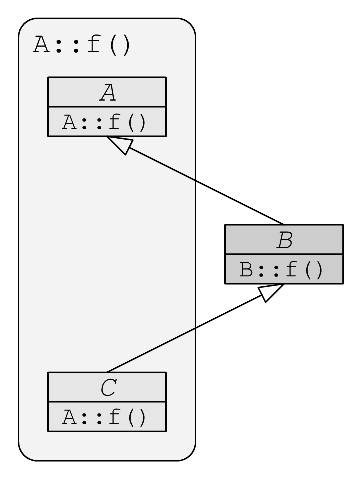
\includegraphics[scale=0.55]{images/fset_failure}}
    \subfigure[][]{\label{fig:fset}\hspace{0.3cm}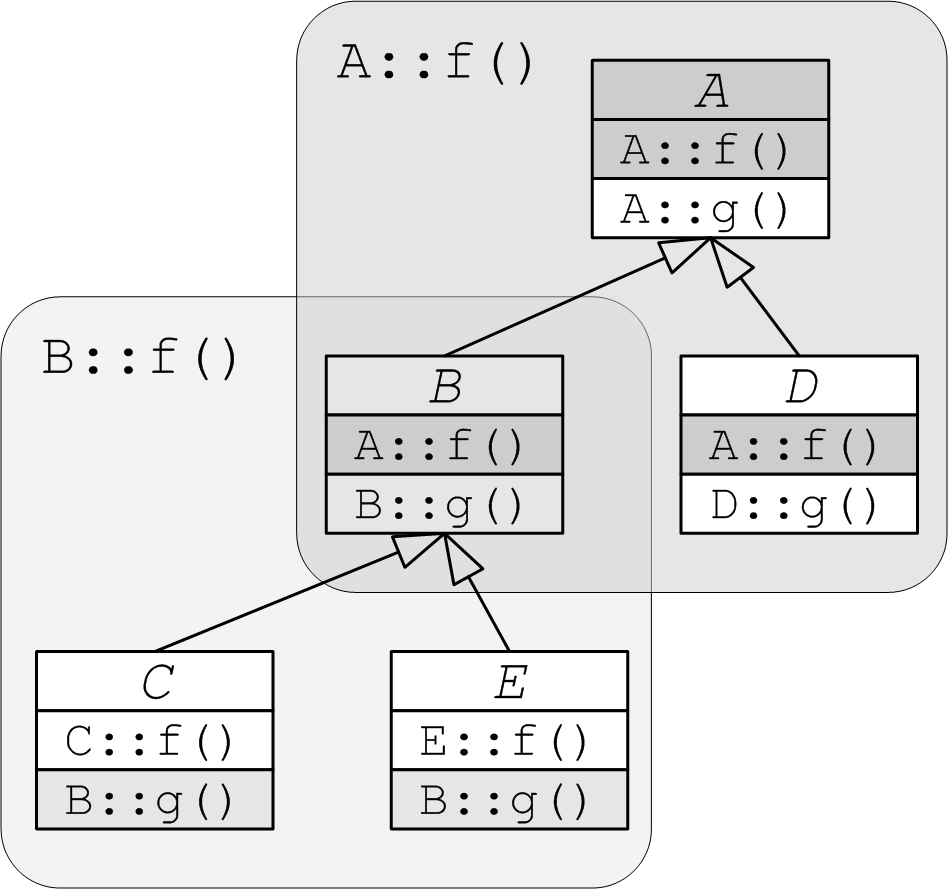
\includegraphics[scale=0.55]{images/fset}}
  \end{center}
\caption{Example for statement~\ref{stmt:fsets_2}.}
\end{figure}

If it is possible to reliably determine the size of the parameters
of a virtual function (for example, if the function uses
a calling convention where the callee clears the stack),
then the following statement holds.
\begin{statement}\label{stmt:param_size}
Let $A, C \in \gC, i \ge 0: |\params(A_i^{\func})| \ne |\params(C_i^{\func})|$.
Then restriction $\cR_{\ref{stmt:param_size}} = \neg (A \sim C)$ is satisfied.
\end{statement}
In compliance with the C++ inheritance rules \cite{cpp03},
a virtual function cannot be overridden by a function with different parameters.

Some information on relation $\leftarrow$ can also be gathered
using an analysis of destructors and constructors.
A constructor of a class performs the following sequence
of operations \cite{cpp03, gray94}:
\begin{enumerate}\compact
\item Calls constructors of direct base classes.
\item Calls constructors of data members.
\item Initializes virtual function table pointer field(s).
\item Performs user-specified initialization code in the body
of the constructor.
\end{enumerate}

So, in case of a ``deep'' inheritance hierarchy,
a construction of an object may require many
successive initializations of the class's virtual function table pointer.
Where appropriate, these assignments are optimized away by the compiler,
but the last assignment is never optimized away.
Conversely, a destructor must deinitialize the object
in the exact reverse order to how it was initialized:
\begin{enumerate}\compact
\item Initializes the virtual function table pointer field(s).
\item Performs user-specified destruction code in the body of the destructor.
\item Calls destructors of data members.
\item Calls destructors of direct bases.
\end{enumerate}

Destruction of an object may also require many successive
initializations of the class's virtual function table pointer.
Experiments have shown that neither GCC nor MSVC optimize away
the last initialization.
That means that the destructor of the object always overwrites
the virtual function table pointer field with a pointer
to a ``most-base'' virtual table.
The inheritance reconstruction method presented in this paper
highly relies on this fact.

Constructors and a destructor are the only functions
that access the virtual function table pointer field of a class.
By analyzing these accesses, it is possible to find bases
of a given virtual table,
%Consider the following construct to appear
%in a virtual function of class \lstinline{SomeClass}:
%\begin{lstlisting}
%new (this) SomeOtherClass(/* ... */)
%\end{lstlisting}
%
%Such construct will overwrite a virtual function table pointer
%of an object of class \lstinline{SomeClass} with a pointer
%to a virtual function table of a possibly unrelated class
%\lstinline{SomeOtherClass}.
%It is hard to imagine where such construct could be useful.
%The fact that it does not appear in the source code of virtual functions
%of some virtual function table $D$ means that inside virtual functions
%of $D$ virtual function table pointer field can be overwritten
%only with a call to destructor.
%In case the above-mentioned construct does not appear in the source code,
so the following statement holds.
\begin{statement}\label{stmt:destructors}
Let $B, D \in \gC: B \ne D$ and
$i \ge 0: D_i^{\func} \enspace \executes \enspace $ \lstinline{*(void**)((char*)this - } $D_i^{\adj}$\lstinline{)} = \lstinline{&}$B$.
Then restriction $\cR_{\ref{stmt:destructors}} = B \lhd D$ is satisfied.
\end{statement}

In compliance with the ABIs used by GCC and MSVC compilers
\cite{gccabi, gray94}, \lstinline{this} pointer passed to a virtual function
always points to a field containing pointer
to the virtual function table corresponding to this function.
Therefore the statement \lstinline{*(void**)((char*)this - } $D_i^{\adj}$ \lstinline{)} = \lstinline{&}$B$ means
that the virtual function table pointer corresponding to virtual table $D$
is overwritten with a pointer to a virtual table $B$.
According to the actions that must be performed by a destructor,
in this case $B \lhd D$.
Moreover, since virtual function table pointer can be overwritten
only in a call to destructor,
the order in which it is overwritten with different
virtual function table pointers actually defines
the inheritance relation $\lhd$ between all these virtual tables.

Since most of the polymorphic class hierarchies use virtual destructors,
in most cases statement \ref{stmt:destructors} will produce
at least one relation $\lhd$~--- between the virtual function
table being analyzed and the ``most-base'' one.

The virtual function table pointer assignments can be detected
via data flow analysis.
In case calling conventions of a virtual function are known,
the way \lstinline{this} pointer is passed to a function is also known,
and data flow analysis can be used to find such assignments.

%\subsection{Definition of a problem of inheritance hierarchy reconstruction}\label{chapter:problem}
\subsection{Inheritance hierarchy reconstruction}
\label{chapter:problem}

As it was denoted in chapter \ref{ch:retrieving},
for each virtual table $D$ with a virtual destructor,
a $B \lhd D$ relation can be reconstructed using
statement \ref{stmt:destructors},
where $B$ is the ``most-base'' virtual table of $D$.
Therefore, using statement \ref{stmt:destructors},
it is possible to construct a set of all virtual tables
in a single connected inheritance hierarchy with virtual destructors.
In a rare case when virtual destructors are not used,
this set can still be restored in most cases using statement \ref{stmt:fsets_2}.
This makes possible to subdivide set $\gC$ into several sets of virtual tables,
so that all virtual tables in a single set
form a connected inheritance hierarchy.
Since we do not consider virtual inheritance, such hierarchy is a rooted tree.
Further in this paper we presume that $\gC$ is one of such sets,
i.e. virtual tables in $\gC$ form an inheritance tree.

Let $\gR \subset \nT^R(\gC) \rightarrow \{0, 1\}$ be a set
of all restrictions on the inheritance tree,
obtained by applying statements \ref{stmt:vtable_size},
\ref{stmt:inherit_pure}, \ref{stmt:fsets_2},
\ref{stmt:param_size}, and \ref{stmt:destructors},
where $\nT^R(X)$ is a set of all rooted trees with nodes from $X$.
Let the function \isSol~for the given rooted tree with nodes from $\gC$ and
a set of restrictions return whether this tree satisfies all
the given restrictions. 
%Let
%\begin{equation}
%\begin{aligned}
%& \isSol \in \nT^R(\gC) \times 2^{\nT^R(\gC) \rightarrow \{0, 1\}} \rightarrow \{0, 1\} \text{,} \\
%& \forall T \in \nT^R(\gC), \gR \in 2^{\nT^R(\gC) \rightarrow \{0, 1\}}: \isSol(T, \gR) \Longleftrightarrow \\
%& \quad \forall \cR \in \gR: \cR(T)\text{.}
%\end{aligned}
%\end{equation}
Then a problem of virtual table hierarchy reconstruction can be considered
as follows:
\begin{equation}\label{eq:problem}
\text{Find~} T \in \nT^R(\gC): \isSol(T, \gR) \text{.}
\end{equation}

Since we have made some assumption on the structure of the source C++ program,
it may be possible that all restrictions from $\gR$ cannot
be jointly satisfied.
That's why we will be solving the relaxed problem:
\begin{equation}\label{eq:relaxed_problem}
\begin{aligned}
& \text{Find~} \gR' \subseteq \gR, T \in \nT^R(\gC): \isSol(T, \gR') \, \wedge \\
& \quad \forall \cR \in \gR \setminus \gR': \nexists T \in \nT^R(\gC): \isSol(T, \gR' \cup \{\cR\})
\end{aligned}
\end{equation}

%\subsection{Building a partial solution of the problem of inheritance hierarchy reconstruction}
\subsection{Building a partial solution}

We assume restrictions $\cR_{\ref{stmt:fsets_2}}$ to be jointly satisfiable.
If they are not, which is a rare case,
additional manual analysis will be required.

Let $\gF$ be the set of all sets $\gf$ from
restrictions $\cR_{\ref{stmt:fsets_2}}$.
Then $\forall \gf \in \gF: \isSol(T, \gR) \Longrightarrow T[\gf] \in \nT(\gf)$,
i.e. a reduction of a solution tree on any of the sets $\gf \in \gF$ is a tree.
Let the function \isPartSol~for the given rooted tree with nodes from $\gC$
and a set of subsets of $\gC$ return whether the reduction of this tree
on all of these subsets is a tree. 
%\begin{equation}\label{eq:is_partial_solution}
%\begin{aligned}
%& \isPartSol \in \nT(\gC) \times 2^{2^{\gC}} \rightarrow \{0, 1\} \text{,}\\
%& \forall T \in \nT(\gC), \gF \in 2^{2^{\gC}}: \isPartSol(T, \gF) \Longleftrightarrow \\
%& \quad \forall \gf \in \gF: T[\gf] \in \nT(\gf)\text{.}
%\end{aligned}
%\end{equation}
Then $\isSol(T, \gR) \Longrightarrow \isPartSol(T, \gF)$. Let
\begin{equation}\label{eq:f_star_def}
\gFs = \bigcup_{\gF' \subseteq \gF} \left\{ \bigcap_{\gf \in \gF'} \gf \right\} \cup \{\gC\} \cup \bigcup_{C \in \gC}\{\{C\}\} \setminus \emptyset \text{,}
\end{equation}
i.e. $\gFs$ is an intersection closure of set $\gF$
with some additional elements.
For $\gFs$ the following condition is satisfied:
\begin{equation}\label{lemma:f_closure_tree}
\forall T \in \nT(\gC): \isPartSol(T, \gF) \Longrightarrow \isPartSol(T, \gFs) \text{.}
\end{equation}

Consider a $\subset$ relation on set $\gFs$.
This relation defines a strict partial order on $\gFs$,
and a Hasse diagram can be constructed for it.
A Hasse diagram is a directed graph representation of
a partially ordered set in which each element is represented by a node.
Immediate successors of each element are connected
to the corresponding node by a directed edge \cite{lerma04}.
Let $\gH$ be a Hasse diagram for $(\gFs, \subset)$,
and $\gH_E$ be a set of all edges of $\gH$,
i.e. if $(\gf_1, \gf_2) \in \gH_E$ then $\gf_1 \subset \gf_2$.
We consider nodes of Hasse diagram $\gH$ to be sets $\gf \in \gFs$.

\if 0
\begin{figure}[htb!]
\begin{algorithmic}[1]
\STATE $T_E = \emptyset$
\FORALL{$\gf \in \gFs$}
    \STATE $\gD \gets \{\gf' \in \gFs | (\gf', \gf) \in \gH_E\}$
    \STATE $\gK \gets \gD$
    \WHILE{$\exists \gf_1, \gf_2 \in \gK: \gf_1 \cap \gf_2 \ne \emptyset$}
        \STATE $\gK \gets \gK \setminus \{\gf_1, \gf_2\} \cup \{\gf_1 \cup \gf_2\}$
    \ENDWHILE
    \STATE $t \gets \any(\nT(\gK))$
    \FORALL{$\{\gf_1, \gf_2\} \in t_E$}
        \STATE $T_E \gets T_E \cup \{\any(\gf_1), \any(\gf_2)\}$
    \ENDFOR
\ENDFOR
\RETURN $T = (\gC, T_E)$
\end{algorithmic}
\caption{Algorithm of building a partial solution tree.}
\label{alg:build_tree}
\end{figure}
\fi

\begin{figure}[htb!]
\small
\begin{minipage}[b]{0.5\textwidth}
\begin{algorithm}{BuildPartialSolution}{
    \label{alg:build_tree}
    \qoutput{Tree that is a partial solution of problem (\ref{eq:relaxed_problem})}
}
$T_E \gets \emptyset$ \\
\qfor \textbf{all} $\gf \in \gFs$ \qdo \\
    $\gD \gets \{\gf' \in \gFs | (\gf', \gf) \in \gH_E\}$ \\
    $\gK \gets \gD$ \\
    \qwhile $\exists \gf_1, \gf_2 \in \gK: \gf_1 \cap \gf_2 \ne \emptyset$ \qdo \\
        $\gK \gets \gK \setminus \{\gf_1, \gf_2\} \cup \{\gf_1 \cup \gf_2\}$
    \qelihw \\
    $t \gets \any(\nT(\gK))$ \\
    \qfor \textbf{all} $\{\gf_1, \gf_2\} \in t_E$, where $t_E$ is a set of edges of $t$ \qdo \\
        $T_E \gets T_E \cup \{\any(\gf_1), \any(\gf_2)\}$
    \qrof
\qrof \\
\qreturn tree $(\gC, T_E)$
\end{algorithm}
\end{minipage}
\end{figure}


Algorithm \ref{alg:build_tree} builds a partial solution
of a relaxed problem (\ref{eq:relaxed_problem}).
For this algorithm the following theorem can be proven.
\begin{theorem}\label{theorem:evil}
If $\exists T' \in \nT(\gC): \isPartSol(T', \gFs)$,
then regardless of the values returned by functions $\any$,
algorithm \ref{alg:build_tree} builds
a tree $T \in \nT(\gC): \isPartSol(T, \gFs)$.
\end{theorem}
\begin{proof}
This theorem can be proven by induction.
Let $T$ be some tree built using algorithm \ref{alg:build_tree}.
If for all sets $\gf_i \in \gFs: \gf_i \subseteq \gf$,
condition $T[\gf_i] \in \nT(\gf_i)$ is satisfied,
then it is also satisfied for $\gf$,
i.e. $T[\gf] \in \nT(\gf)$.
Since $\gC \in \gFs$, condition $\isPartSol(T, \gFs)$ will also be met.

The base of induction is $|\gf| = 1$.
The induction step can be proven from the contrary,
assuming that there is a cycle in $T[\gf]$.
In this case cycle will also be present in $T'$,
which contradicts the hypothesis of the theorem.
\end{proof}

A consequence of this theorem is that under the additional requirement
that all the restrictions $\cR_{\ref{stmt:fsets_2}}$ must be jointly satisfied,
any solution of problem (\ref{eq:relaxed_problem})
can be generated using algorithm \ref{alg:build_tree}.

%\subsection{Building a complete solution of the problem of inheritance hierarchy reconstruction}
\subsection{Building a complete solution}
\label{chapter:full_reconstruction}

For each node $\gf$ of Hasse diagram $\gH$ algorithm \ref{alg:build_tree}
builds set $\gD$.
We call this set a set of \textit{child nodes} for node $\gf$.
For each node $\gf$ algorithm \ref{alg:build_tree} also builds set $\gK$.
Let $\gFu$ be a union of sets $\gK \setminus \gD$ for all nodes
of Hasse diagram $\gH$.
Let $\gG$ be a Hasse diagram for $(\gFs \cup \gFu, \subset)$,
and let all the nodes of this graph be divided into two types~---
$\any$-nodes and $\fixed$-nodes.
Node $\gf$ is a $\fixed$-node, if $\gf \in \gFu$,
and an $\any$-node, if $\gf \in \gFs$.
Note that each two child nodes of a $\any$-node have empty intersection,
and each two child nodes of a $\fixed$-node have non-empty intersection.
That means that if tree $T$ is a partial solution
for problem (\ref{eq:relaxed_problem}),
then for any $\fixed$-node $\gf$ the structure of the tree $T[\gf]$
is fully determined by the structure of corresponding trees of its children,
while for each $\any$-node $\gf'$ the structure of the tree $T[\gf']$
is defined by the return values of functions $\any$
in algorithm \ref{alg:build_tree}.

Fig. \if 0 \ref{fig:gg_tree} \fi 2 illustrates
the difference between graphs $\gH$ and $\gG$.
On Fig. \ref{fig:gg_example} a fragment of graph $\gG$ is presented
that corresponds to the fragment of graph $\gH$
presented on Fig. \ref{fig:gh_example}.

\begin{figure}[htb!]
\centering
  \begin{center}
    \subfigure[][]{\label{fig:gh_example}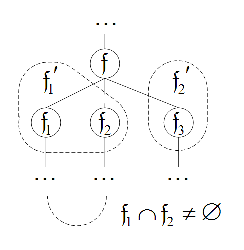
\includegraphics[scale=1.2]{images/gg_algo_class}}
    \subfigure[][]{\label{fig:gg_example}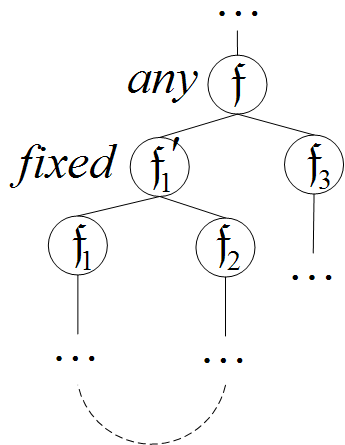
\includegraphics[scale=1.2]{images/gg_algo_class_2}}
  \end{center}
\label{fig:gg_tree}
%\caption{Example of corresponding fragments of graphs $\gH$ and $\gG$.}
\caption{Fragments of graphs $\gH$ and $\gG$.}
\end{figure}

Solution of the problem (\ref{eq:relaxed_problem})
is constructed using graph $\gG$.
The following functions will be used:

$\children$ --- returns the set of child nodes for the given node $\gf$.

$\type$ --- returns the type of the given node, $\any$ or $\fixed$.

$\vtable$ --- if for the given node $\gf$ condition $|\gf| = 1$ is satisfied,
then returns $\gf$, else returns $\emptyset$.

$\adjacent$ --- for the given node returns the set
of adjacent nodes in graph $\gG$.

$\parents$ --- returns the set of adjacent non-child nodes for the given node,
i.e. $\parents(\gf) = \adjacent(\gf) \setminus \children(\gf)$.
Note that if $\type(\gf) = \fixed$,
then there is only one node in $\parents(\gf)$.

Graph $\gG$ is constructed so that there are no cycles of $\any$-nodes in $\gG$.
Also for each $\any$-node:
\begin{equation}\label{eq:number_of_children}
|\children(\gf)| \le |\gC| \text{,}
\end{equation}

Let set $\gC'_{(\gf_1, \gf_2)}$,
where $\gf_1$ and $\gf_2$ are two adjacent nodes in $\gG$,
be the set of all reachable virtual tables in the direction
from $\gf_1$ to $\gf_2$.
It is defined as follows:
\begin{equation}\label{eq:cset_for_class}
\begin{aligned}
&\type(\gf_1) = \type(\gf_2) = \any \wedge \vtable(\gf_2) \ne \emptyset \\
&\quad \Longrightarrow \gC'_{(\gf_1, \gf_2)} = \vtable(\gf_2) \text{.}
\end{aligned}
\end{equation}

Else, if 
%the following condition is met:
%\begin{equation}\label{eq:cset_for_rest_cond}
%begin{aligned}
%&( \type(\gf_1) = \type(\gf_2) = \any ) \vee \\
%&( \exists \{\gf'_1, \gf'_2\} = \{\gf_1, \gf_2\}: \type(\gf'_1) = \any \\
%&\quad \wedge \type(\gf'_2) = \fixed \wedge \parents(\gf'_2) = \{\gf'_1\} ) \text{,}
%\end{aligned}
%\end{equation}
%i.e. 
$\gf_1$ and $\gf_2$ are $\any$-nodes,
or one of the nodes $\gf_1$ and $\gf_2$ is a $\fixed$-node,
and the other one is an $\any$-node,
and $\fixed$-node is a child of $\any$-node, then:
\begin{equation}\label{eq:cset_for_rest}
\gC'_{(\gf_1, \gf_2)} = \bigcup_{\gf \in \adjacent(\gf_2) \setminus \gf_1} \gC'_{(\gf_2, \gf)} \text{.}
\end{equation}

In case neither of the two conditions are met,
$\gC'_{(\gf_1, \gf_2)}$ is empty.
Since there are no cycles of $\any$-nodes in $\gF$,
recursive definition (\ref{eq:cset_for_rest}) is correct.

For any two nodes $\gf_1$ and $\gf_2$
let $\gC_{(\gf_1, \gf_2)} = \gC'_{(\gf_1, \gf_2)}$
with the additional condition that if $\gf_1$ is an $\any$-node,
and $\gf_2$ is the closest to $\gf_1$ direct or indirect parent $\fixed$-node,
then:
\begin{equation}
\gC_{(\gf_1, \gf_2)} = \gC \setminus \left( \vtable(\gf_1) \cup \bigcup_{\gf \in \gC} \gC'_{(\gf_1, \gf)} \right) \text{.}
\end{equation}

Then the following conditions are met:
\begin{equation}\label{eq:gc_props}
\begin{aligned}
&\forall \gf \in \gG_V: \bigcup_{\gf' \in \gG_V} \gC_{(\gf, \gf')} = \gC \setminus \vtable(\gf) \text{,} \\
&\forall \gf_1, \gf_2 \in \gG_V: \gC_{(\gf, \gf_1)} \cap \gC_{(\gf, \gf_2)} = \emptyset \text{,}
\end{aligned}
\end{equation}
where $\gG_V$ is the set of all nodes of graph $\gG$.

%A solution of (\ref{eq:relaxed_problem}) is constructed as a rooted tree $T \in \nT^R(\gC)$. This tree is with an algorithm \ref{alg:build_tree}, but with functions $\any$ returning predefined values. Such tree is a partial solution due to theorem \ref{theorem:evil}.

The presented algorithm iteratively builds the following sets
for each two child nodes $\gf_1$ and $\gf_2$ of each $\any$-node $\gf \in \gG$:

$\gN^{\gf}_{(\gf_1, \gf_2)}$ --- the set of virtual tables,
that must be inherited by the root of $T[\gf_1]$
in case its base lies in $\gf_2$,
where $T$ is a solution of problem \ref{eq:relaxed_problem}.

$\gP^{\gf}_{(\gf_1, \gf_2)}$ --- the set of virtual tables,
that must not be inherited by the root of $T[\gf_1]$
in case its base lies in $\gf_2$.

For these sets the following condition is satisfied:
\begin{equation}\label{eq:gn_gp_in_gc}
\gP^{\gf}_{(\gf_1, \gf_2)}, \gN^{\gf}_{(\gf_1, \gf_2)} \subseteq \gC_{(\gf_1, \gf_2)}
\end{equation}

The presented algorithm also works with an $\lhd$ relation
defined on the set of child nodes of each $\any$-node $\gf$.
In case $\gf_1$ and $\gf_2$ are child nodes of $\gf$, $\gf_1 \lhd \gf_2$
means that the base of the root of $T[\gf_2]$ lies in $\gf_1$.
For each $\any$-node $\gf$ relation $\lhd$ must define
a rooted tree $T_{\gf} \in \nT^R(\children(\gf))$.
Let this relation be described with a set of restrictions $\gR_{\gf}$
of the following form:
\begin{equation}\label{eq:restriction_type}
\begin{aligned}
\cR &= b \nrhd d \text{, or} \\
\cR &= a \sim c \text{.}
\end{aligned}
\end{equation}
Restrictions $\cR = \neg (a \sim c)$ can be represented
as two restrictions $\cR_\nrhd = a \nrhd c$ and $\cR_\nlhd = a \nlhd c$.
Restrictions $\cR = a \lhd c$ can also be represented
as two restrictions $\cR_\nrhd = a \nrhd c$ and $\cR_{\sim} = a \sim c$.

All restrictions from $\gR$,
except for restrictions $\cR_{\ref{stmt:fsets_2}}$,
can also be represented in the form (\ref{eq:restriction_type}).
Let $\gR_s \subseteq \gR$~--- the set of all restrictions from $\gR$,
except for restrictions $\cR_{\ref{stmt:fsets_2}}$.

As it was denoted at the end of chapter \ref{chapter:problem},
not all of the restrictions from $\gR$ may be jointly satisfiable.
Therefore, solution tree $T$ is built by considering restrictions
from $\gR_s$ one by one.
In case the restriction results in a conflict and construction
of the solution tree become impossible,
the last step of the algorithm is undone,
and the restriction under consideration is added to set $\gR_{\times}$.
After processing all restrictions,
set $\gR \setminus \gR_{\times}$ corresponds
to set $\gR'$ from definition of the relaxed problem (\ref{eq:relaxed_problem}).

\if 0
\begin{figure}[htb!]
\begin{algorithmic}[1]
\STATE \textbf{let} $\cR \in \gR_s, A, C \in \gC: A \ne C \wedge \cR = A \sim C$
\STATE \textbf{let} $\gf_1: \vtable(\gf_1) = \{C\}$
\WHILE{$\vtable(\gf_1) \ne \{A\}$}
    \STATE \COMMENT{Due to (\ref{eq:gc_props}) there is only one $\gf_2$}
    \STATE \textbf{let} $\gf_2 \in \adjacent(\gf_1): A \in \gC_{(\gf_1, \gf_2)}$
    \IF{$\type(\gf_2) = \any \wedge \gf_1 \in \children(\gf_2) \wedge \exists \gf_3 \in \children(\gf_2): B \in \gC_{(\gf_2, \gf_3)}$}
        \STATE $\gN^{\gf_2}_{(\gf_1, \gf_3)} \gets \gN^{\gf_2}_{(\gf_1, \gf_3)} \cup \{C\}$
        \STATE $\gN^{\gf_2}_{(\gf_3, \gf_1)} \gets \gN^{\gf_2}_{(\gf_3, \gf_1)} \cup \{A\}$
    \ELSIF{$\type(\gf_2) = \fixed \wedge \gf_2 \in \children(\gf_1)$}
        \STATE \textbf{break}
    \ENDIF
    \STATE $\gf_1 \gets \gf_2$
\ENDWHILE
\end{algorithmic}
\caption{Algorithm for handling restrictions of the type $A \sim C$.}
\label{alg:process_sim}
\end{figure}

\begin{figure}[htb!]
\begin{algorithmic}[1]
\STATE \textbf{let} $\cR \in \gR_s, B, D \in \gC: B \ne C \wedge \cR = B \nrhd D$
\STATE \textbf{let} $\gf_1: \vtable(\gf_1) = \{D\}$
\WHILE{$\vtable(\gf_1) \ne \{B\}$}
    \STATE \COMMENT{Due to (\ref{eq:gc_props}) there is only one $\gf_2$}
    \STATE \textbf{let} $\gf_2 \in \adjacent(\gf_1): B \in \gC_{(\gf_1, \gf_2)}$
    \IF{$\type(\gf_2) = \any \wedge \gf_1 \in \children(\gf_2) \wedge \exists \gf_3 \in \children(\gf_2): B \in \gC_{(\gf_2, \gf_3)}$}
        \STATE $\gN^{\gf_2}_{(\gf_1, \gf_3)} \gets \gN^{\gf_2}_{(\gf_1, \gf_3)} \cup \{B\}$
        \STATE $\gP^{\gf_2}_{(\gf_3, \gf_1)} \gets \gP^{\gf_2}_{(\gf_3, \gf_1)} \cup \{D\}$
    \ELSIF{$\type(\gf_2) = \fixed \wedge \gf_2 \in \children(\gf_1)$}
        \STATE \textbf{break}
    \ENDIF
    \STATE $\gf_1 \gets \gf_2$
\ENDWHILE
\end{algorithmic}
%\caption{Algorithm for handling restrictions of the type $B \nrhd D$.}
\caption{Handling restrictions of the type $B \nrhd D$.}
\label{alg:process_less}
\end{figure}
\fi

\begin{figure}[htb!]
\small
\begin{minipage}[b]{0.47\textwidth}
\begin{algorithm}{ProcessSim}{
    \label{alg:process_sim}
    \qinput{Virtual tables $A, C \in \gC: A \sim C \in \gR$}
}
\textbf{let} $\gf_1: \vtable(\gf_1) = \{C\}$ \\
\qwhile $\vtable(\gf_1) \ne \{A\}$ \qdo \\
    \qcom{Due to (\ref{eq:gc_props}) there exists only one set $\gf_2$} \\
    \textbf{let} $\gf_2 \in \adjacent(\gf_1): A \in \gC_{(\gf_1, \gf_2)}$ \\
    \qif $\type(\gf_2) = \any \wedge \gf_1 \in \children(\gf_2) \wedge \exists \gf_3 \in \children(\gf_2): B \in \gC_{(\gf_2, \gf_3)}$ \qthen \\
        $\gN^{\gf_2}_{(\gf_1, \gf_3)} \gets \gN^{\gf_2}_{(\gf_1, \gf_3)} \cup \{C\}$ \\
        $\gN^{\gf_2}_{(\gf_3, \gf_1)} \gets \gN^{\gf_2}_{(\gf_3, \gf_1)} \cup \{A\}$ \\
    \qelseif $\type(\gf_2) = \fixed \wedge \gf_2 \in \children(\gf_1)$ \qthen \\
        \textbf{break}
    \qfi \\
    $\gf_1 \gets \gf_2$
\qelihw
\end{algorithm}
\end{minipage}
\end{figure}

\begin{figure}[htb!]
\small
\begin{minipage}[b]{0.47\textwidth}
\begin{algorithm}{ProcessNotDerived}{
    \label{alg:process_less}
    \qinput{Virtual tables $B, D \in \gC: B \nrhd D \in \gR$}
}
\textbf{let} $\gf_1: \vtable(\gf_1) = \{D\}$ \\
\qwhile $\vtable(\gf_1) \ne \{B\}$ \qdo \\
    \qcom{Due to (\ref{eq:gc_props}) there exists only one set $\gf_2$} \\
    \textbf{let} $\gf_2 \in \adjacent(\gf_1): B \in \gC_{(\gf_1, \gf_2)}$ \\
    \qif $\type(\gf_2) = \any \wedge \gf_1 \in \children(\gf_2) \wedge \exists \gf_3 \in \children(\gf_2): B \in \gC_{(\gf_2, \gf_3)}$ \qthen \\
        $\gN^{\gf_2}_{(\gf_1, \gf_3)} \gets \gN^{\gf_2}_{(\gf_1, \gf_3)} \cup \{B\}$ \\
        $\gP^{\gf_2}_{(\gf_3, \gf_1)} \gets \gP^{\gf_2}_{(\gf_3, \gf_1)} \cup \{D\}$ \\
    \qelseif $\type(\gf_2) = \fixed \wedge \gf_2 \in \children(\gf_1)$ \qthen \\
        \textbf{break}
    \qfi \\
    $\gf_1 \gets \gf_2$
\qelihw
\end{algorithm}
\end{minipage}
\end{figure}


The reconstruction algorithm starts
with all sets $\gR_{\gf}$, $\gN^{\gf}_{(\gf_1, \gf_2)}$
and $\gP^{\gf}_{(\gf_1, \gf_2)}$ being empty.
It continuously processes restrictions from $\gR_s$ with
one of algorithms \ref{alg:process_sim} and \ref{alg:process_less},
and then modifies the sets to be consistent.
Following are consistency maintenance rules.

Let $\gf$ be an $\any$-node,
and $\gf_1$, $\gf_2$ and $\gf_3$ be child nodes of $\gf$.
Then from the definition of $\gN^{\gf}_{(\gf_1, \gf_2)}$ and $\sim$:
\begin{equation}\label{eq:gf_consistency_1}
\begin{aligned}
&\gN^{\gf}_{(\gf_1, \gf_2)} \ne \emptyset \wedge \gN^{\gf}_{(\gf_2, \gf_1)} \ne \emptyset \\
&\quad \Longrightarrow (\gf_1 \sim \gf_2) \in \gR_{\gf}
\end{aligned}
\end{equation}

Sets $\gP^{\gf}_{(\gf_1, \gf_2)}$ and $\gN^{\gf}_{(\gf_1, \gf_2)}$ must not conflict:
\begin{equation}\label{eq:gf_consistency_2}
\begin{aligned}
&\gP^{\gf}_{(\gf_1, \gf_2)} \cap \gN^{\gf}_{(\gf_1, \gf_2)} \ne \emptyset \\
&\quad \Longrightarrow (\gf_1 \nrhd \gf_2) \in \gR_{\gf}
\end{aligned}
\end{equation}

After applying rules (\ref{eq:gf_consistency_1})
and (\ref{eq:gf_consistency_2}), sets $\gR_{\gf}$ may have been modified.
For elements of these sets the following consistency maintenance rules are used:
\begin{equation}\label{eq:consistency_gr}
\begin{aligned}
&b \lhd d \Longleftrightarrow b \nrhd d \wedge b \sim d \\
&b \lhd c \wedge c \lhd d \Longrightarrow b \lhd d \\
&d_1 \sim d_2, \ldots, d_{n - 1} \sim d_n, d_n \sim d_1 \Longrightarrow \\
&\quad \forall a, c \in \{d_1, \ldots, d_n\}: a \sim c
\end{aligned}
\end{equation}
These rules are based on the properties of relations $\nrhd$, $\lhd$
and $\sim$, and on the fact that they must define
a tree on $\children(\gf)$.
Also there must be no conflicts in $\gR_{\gf}$,
i.e. the following condition must be met:
\begin{equation}\label{eq:consistency_conflict_1}
\neg(b \sim d \wedge b \nlhd d \wedge b \nrhd d)
\end{equation}

After applying rules (\ref{eq:consistency_gr}),
additional consistency maintenance rules for sets $\gR_{\gf}$ are applied.
Two unrelated virtual tables cannot be base for a single virtual table,
and therefore:
\begin{equation}\label{eq:gca_consistency_1}
\begin{aligned}
&\{\gf_1 \rhd \gf_2\} \subseteq \gR_{\gf}, A, C \in \gN^{\gf}_{(\gf_1, \gf_2)}: A \ne C \\
&\quad \Longrightarrow A \sim C
\end{aligned}
\end{equation}

There are no cycles of $\any$-nodes in $\gG$, and therefore:
\begin{equation}\label{eq:gca_consistency_2}
\begin{aligned}
&\{\gf_1 \rhd \gf_2\} \subseteq \gR_{\gf}, B \in \gN^{\gf}_{(\gf_1, \gf_2)}, D \in \gC_{(\gf, \gf_1)} \\
&\quad \Longrightarrow D \rhd B
\end{aligned}
\end{equation}

In case $\{\gf_1 \rhd \gf_2\} \subseteq \gR_{\gf}$,
it must be possible to inherit from $T[\gf_2]$
all virtual tables $\gN^{\gf}_{(\gf_1, \gf_2)}$
without inheriting any of virtual tables $\gP^{\gf}_{(\gf_1, \gf_2)}$:
\begin{equation}\label{eq:gca_consistency_3}
\begin{aligned}
&\{\gf_1 \rhd \gf_2\} \subseteq \gR_{\gf}, B \in \gN^{\gf}_{(\gf_1, \gf_2)}, D \in \gP^{\gf}_{(\gf_1, \gf_2)} \\
&\quad \Longrightarrow D \nlhd B
\end{aligned}
\end{equation}

The outline of the algorithm is as follows:
\begin{enumerate}
\renewcommand{\theenumii}{\arabic{enumii}}
\renewcommand{\labelenumii}{\theenumi.\theenumii.}
\item A new restriction $\cR$ from $\gR_s$ is selected.
 It is processed by algorithm \ref{alg:process_sim} or \ref{alg:process_less}.
 \label{item:start}
\item The consistency maintenance rules are applied.
 \label{item:check_consistency}
    \begin{enumerate}
    \item Algorithms \ref{alg:process_sim} and \ref{alg:process_less}
          modify sets $\gN^{\gf}_{(\gf_2, \gf_1)}$ and $\gP^{\gf}_{(\gf_1, \gf_2)}$.
          For modified sets consistency maintenance
          rules (\ref{eq:gf_consistency_1}) and (\ref{eq:gf_consistency_2})
          are applied.
          \label{item:consistency_start}
    \item These consistency maintenance rules modify $\gR_{\gf}$ sets.
          For these sets consistency maintenance
          rules (\ref{eq:consistency_gr}) are applied.
          If consistency criteria (\ref{eq:consistency_conflict_1}) is not met,
          then $\cR$ is added to $\gR_{\times}$,
          all structures are returned to their state on the previous iteration,
          and the algorithm restarts from step \ref{item:start}.
    \item For modified sets $\gR_{\gf}$, consistency maintenance
          rules (\ref{eq:gca_consistency_1}), (\ref{eq:gca_consistency_2}),
          and (\ref{eq:gca_consistency_3}) are applied.
          These rules add new restrictions on virtual tables from $\gC$.
          These restrictions are processed with
          algorithms \ref{alg:process_sim} and \ref{alg:process_less},
          and for these restrictions steps 2.1-2.3 are repeated.
          Since all sets being processed are finite,
          this recursive process will stop.
          \label{item:consistency_end}
    \end{enumerate}
\item It is checked whether for each node $\gf$ there exists
 a rooted tree $T_{\gf} \in \nT^R(\children(\gf))$ satisfying $\gR_{\gf}$.
 If such tree does not exist, then $\cR$ is added to $\gR_{\times}$,
 all structures are returned to their state on the previous iteration,
 and the algorithm restarts from step \ref{item:start}.
 \label{item:check_tree_existence}
\item In case there are unprocessed restrictions in $\gR_s$,
 algorithm restarts from step \ref{item:start}.
\item For each $\any$-node $\gf$,
 rooted tree $T_{\gf} \in \nT^R(\children(\gf))$ satisfying $\gR_{\gf}$
 is constructed.
 Existence of such tree was checked on step
 \ref{item:check_tree_existence}.
\item Trees $T[\gf] \in \nT^R(\gf)$ are constructed for $\any$-nodes
 in an order so that tree for node $\gf$ is constructed
 only when trees for each child node of $\gf$ have already been constructed.
 Each tree $T[\gf]$ and $T_{\gf}$ can be seen as a directed graph
 with edges directed towards the root of this tree.
 \label{item:build_sol}
    \begin{enumerate}
    \item For each directed edge $(\gf_1, \gf_2) \in T_{\gf}$
          an edge connecting root $R$ of $T[\gf_1]$ and a node from $\gf_2$
          is added to $T[\gf]$,
          so that all nodes from $\gN^{\gf}_{(\gf_1, \gf_2)}$ are reachable
          from $R$ via directed edge walk,
          and all nodes from $\gP^{\gf}_{(\gf_1, \gf_2)}$ are not.
          Existence of such edge is ensured by
          rule (\ref{eq:gca_consistency_3}).
    \item If $\gf_R$ is the root of $T_{\gf}$,
          then the root of $T[\gf_R]$ is selected as the root of $T[\gf]$.
    \end{enumerate}
\end{enumerate}

The way the solution tree is built in this algorithm
corresponds to the way it is build in algorithm \ref{alg:build_tree},
and according to theorem \ref{theorem:evil},
this tree satisfies all the restrictions $\cR_{\ref{stmt:fsets_2}}$. Therefore, this tree is the solution of the relaxed problem (\ref{eq:relaxed_problem}).

\subsection{Complexity analysis}

Let $n = |\gC|$, and $N = |\gFs|$.
By definition (\ref{eq:f_star_def}), $N \ge n$.
The number of $\any$-nodes in $\gG$ equals $|\gFs|$,
and due to (\ref{eq:gc_props}),
the total size of all $\gC_{(\gf_1, \gf_2)}$ sets does not exceed $nN$.

Every $\fixed$-node in $\gG$ can only have $\any$-nodes as children. Considering the fact that each $\any$-node can have at most one parent $\fixed$-node, the number of $\fixed$-nodes in $\gG$ does not exceed the number of $\any$-nodes. It means that:
\begin{equation}\label{eq:vertices_in_ggv}
|\gG_V| \le 2N \text{.}
\end{equation}

There are no cycles of $\any$-nodes in $\gG$,
and therefore the number of edges connecting $\any$-nodes in $\gG$
does not exceed $N$.
Since each $\fixed$-node has exactly one parent $\any$-node,
the total number of child nodes of all $\any$-nodes does not exceed $2N$:
\begin{equation}\label{eq:sum_children}
\sum_{\gf \in \gG_V: \type(\gf) = \any} |\children(\gf)| \le 2N \text{.}
\end{equation}

The implication of (\ref{eq:vertices_in_ggv})
is that the total size of all sets corresponding to the vertices of $\gG$
does not exceed $2nN$.
Also (\ref{eq:number_of_children}) and (\ref{eq:sum_children}) imply
that the total number of restrictions in sets $\gR_{\gf}$ does not exceed $4nN$.
Implication of (\ref{eq:gc_props}), (\ref{eq:gn_gp_in_gc}),
and (\ref{eq:sum_children}) is that the total size
of all sets $\gN^{\gf}_{(\gf_1, \gf_2)}$ and $\gP^{\gf}_{(\gf_1, \gf_2)}$
does not exceed $4nN$.
The number of different restrictions of type (\ref{eq:restriction_type})
on $\gC$ does not exceed $2n^2$.
Therefore, memory requirements of the presented algorithm are $O(nN)$.

Estimation of computational complexity of the presented algorithm is given
in an assumption that it rarely performs restarts
with modification of set $\gR_{\times}$,
and these restarts do not affect the total computational complexity.
Set $\gFs$ can be constructed in $O(nN^2)$ operations.
Conditions (\ref{eq:gf_consistency_1})--(\ref{eq:gf_consistency_2})
are checked every time a new element is added to one
of sets $\gN^{\gf}_{(\gf_1, \gf_2)}$ and $\gP^{\gf}_{(\gf_1, \gf_2)}$.
Since the added element is known,
these conditions can be checked in $O(n^2)$ operations.
Conditions (\ref{eq:consistency_gr}), (\ref{eq:consistency_conflict_1}),
(\ref{eq:gca_consistency_1}), (\ref{eq:gca_consistency_2}),
and (\ref{eq:gca_consistency_3}) are checked every time a new element
is added to one of sets $\gR_{\gf}$.
Since the added element is known,
these conditions can also be checked in $O(n^2)$.

Each $\any$-node in $\gG$ can have a single child node
only if this node is a $\fixed$-node.
Therefore, since each time
the algorithms \ref{alg:process_sim} or \ref{alg:process_less} step down
from a parent to a child node,
they either step into a $\fixed$-node and stop,
or step into an $\any$-node,
and that makes the size of set $\gC_{(\gf_1, \gf_2)}$ decrease
on the next iteration of the algorithm.
Due to the fact that the longest path in $\gG$,
where each next node is the parent of the previous one,
is no longer than $n$, and (\ref{eq:gc_props}),
the number of iterations of
algorithms \ref{alg:process_sim} and \ref{alg:process_less}
is no more than $2n$.
Using appropriate data structures, each step of
algorithms \ref{alg:process_sim} and \ref{alg:process_less}
can be performed in $O(\log{n})$,
and therefore the computational complexity of
these algorithms is $O(n \log{n})$.
Since the total number of possible restrictions
of type (\ref{eq:restriction_type}) on set $\gC$
does not exceed $2n^2$,
the total number of restrictions in sets $\gR_{\gf}$
does not exceed $4nN$,
and the total size of
sets $\gN^{\gf}_{(\gf_1, \gf_2)}$ and $\gP^{\gf}_{(\gf_1, \gf_2)}$
does not exceed $4nN$,
the total computational complexity
of steps \ref{item:start}--\ref{item:check_consistency} is $O(n^3N)$.

The check on step \ref{item:check_tree_existence} for a single node
can be performed in $O(n^2)$.
The total number of restrictions in sets $\gR_{\gf}$
does not exceed $4nN$,
and therefore the total computational complexity
of step \ref{item:check_tree_existence} is $O(n^3N)$.

Trees on step \ref{item:build_sol} can be constructed
in $O(n^2)$ operations.
The total of $N$ of such trees must be constructed.
The total of $n - 1$ edges will be added to tree $T$
on step \ref{item:build_sol}.1.
Since each edge can be found in $O(n^2)$ operations,
 the total computational complexity of step \ref{item:build_sol} is $O(n^2N)$

Therefore, the total computational complexity
of the presented algorithm is $O(n^3N)$.
Even though the size of $\gFs$ seem to be growing exponentially of $n$,
experiments have shown that in most cases $N = |\gFs| < n^2$.
Therefore, in most cases the algorithm requires $O(n^3)$ memory
and runs in $O(n^5)$ time.

%Despite the high computational complexity,
%the presented algorithm can be used to solve most of the practical tasks
%related to inheritance hierarchy reconstruction
%in case run-time type information is not present.
%This is because large hierarchies consisting of more than 100 classes,
%like Qt \if 0 \cite{qt} \fi or MFC \if 0 \cite{mfc} \fi,
%normally use run-time type information in one form or another,
%and for such hierarchies it is not needed to use the presented algorithm.

%\subsection{Gathering information on multiple inheritance}
\subsection{Multiple inheritance}

According to the ABIs used by GCC and MSVC compilers \cite{gccabi, gray94},
the virtual function table pointer is always the first field in a class,
and every virtual function expects the passed \lstinline{this} pointer
to point at the beginning of an embedded instance of the class
that first introduced this virtual function.
This means that in case a class defines a function that
must be present in several virtual tables belonging to this class,
only one function body will be generated,
and in all but one of the virtual tables pointers to adjuster thunks
will be stored instead of a pointer to function body.
These adjuster thunks will perform adjustment of the passed \lstinline{this}
pointer, and then pass control to the function body.

Therefore, the following statement holds.
\begin{statement}\label{stmt:multiple_inheritance}
Let $A, C \in \gC, i \ge 0: A_i^{\func} = C_i^{\func} \wedge A_i^{\adj} \ne C_i^{\adj}$.
Then virtual tables $A$ and $C$ belong to two (not necessarily different)
classes that use multiple inheritance and $A_i^{\adj} - C_i^{\adj}$
is an offset between corresponding virtual table pointer fields
in these classes.
\end{statement}

If all bases of class \lstinline{SomeClass} use virtual destructors, then the virtual destructor of this class must be present in all virtual tables of this class, and statement \ref{stmt:multiple_inheritance} can be applied. Most polymorphic class hierarchies use virtual destructors, and that's why the use of multiple inheritance can be detected in most cases by using statement \ref{stmt:multiple_inheritance}. Since destructor of class \lstinline{SomeClass} can be reused in one of derived classes, statement \ref{stmt:multiple_inheritance} cannot be used to reliably determine which virtual tables belong to the same class.

\section{Experimental results}
\label{sectionExperiments}

The presented techniques for inheritance hierarchy reconstruction
were implemented in an application,
a part of which was written in C++, and another part~--- in IDC,
a programming language of the IDA Pro interactive disassembler.
This application was tested on several open source projects,
including doxygen \if 0 \cite{doxygen} \fi
and mkvmerge \if 0 \cite{mkvtoolnix} \fi.
Each of these projects was compiled twice --- with and without
run-time type information.
The created application was used to process the resulting binaries,
and results were compared with the results of source code analysis.

In case run-time type information was used,
the class hierarchy was reconstructed in exactly the same form
as it was present in the source code.
If run-time type information was not present in the assembly,
a set of virtual tables was reconstructed with some function pointers present
in the assembly being mistakenly treated as virtual function tables.
Using the algorithm presented in chapter \ref{chapter:full_reconstruction},
the inheritance relation was correctly reconstructed
on the set of virtual tables that contained virtual destructors.
On most of the virtual tables that did not contain virtual destructors
the inheritance relation was also reconstructed correctly.

\begin{figure}[htb!]
\centering
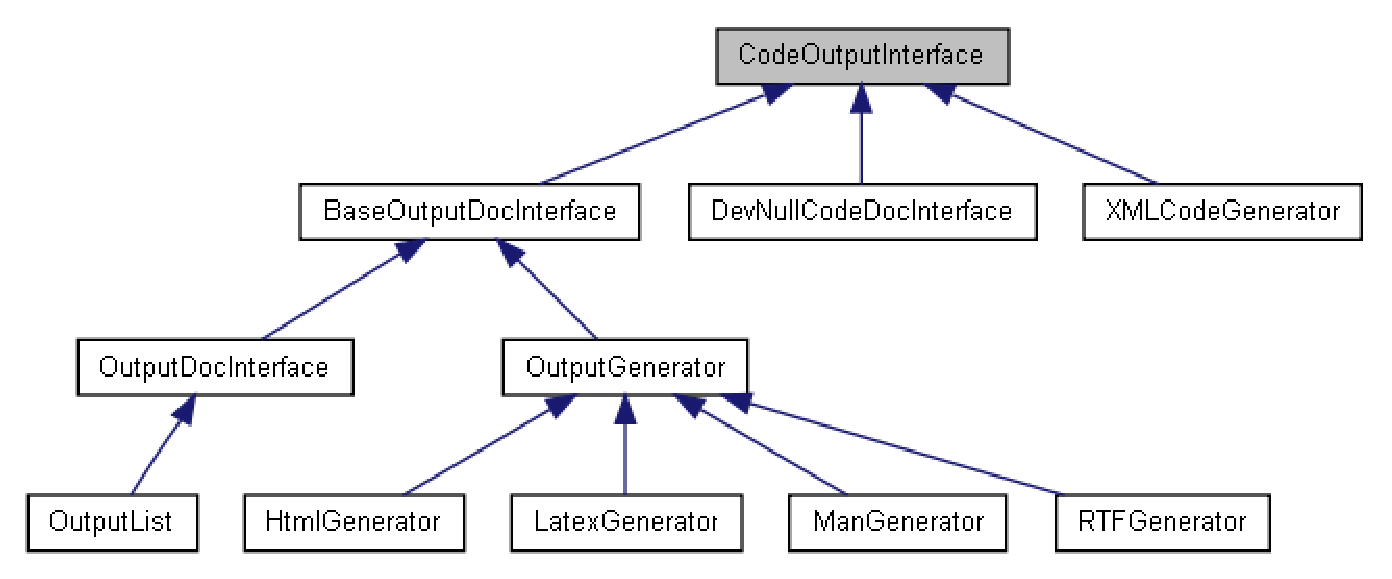
\includegraphics[width=0.5\textwidth]{images/doxy_objtree_doxy}
\caption{Fragment of class hierarchy of doxygen.}
\label{fig:objtree_doxy}
\end{figure}

\begin{figure}[htb!]
\centering
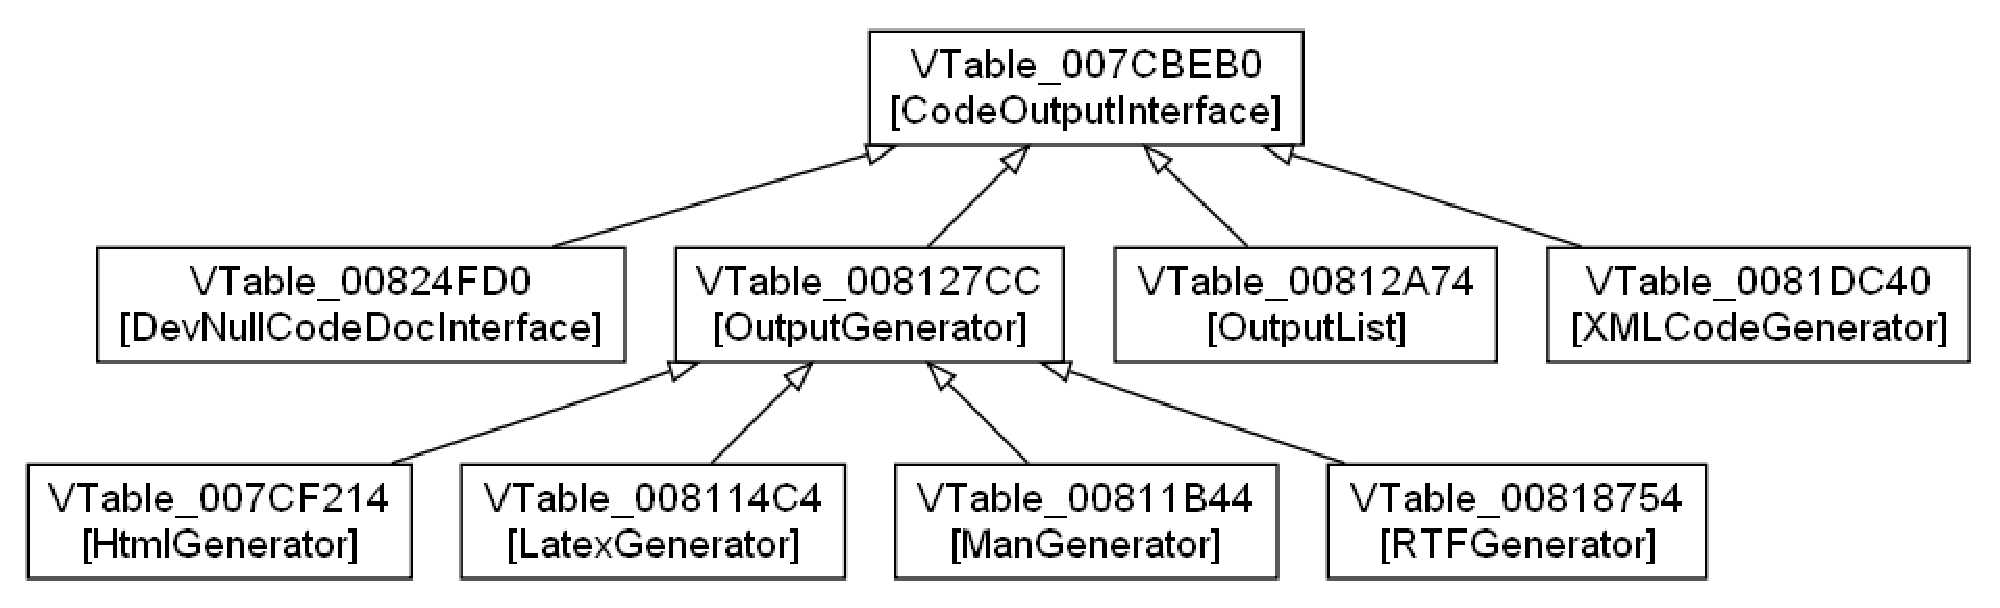
\includegraphics[width=0.5\textwidth]{images/doxy_objtree_nortti_label}
\caption{Fragment of reconstructed virtual table hierarchy.}
\label{fig:objtree_our}
\end{figure}

Fig.~\ref{fig:objtree_our} demonstrates the inheritance relation
on the set of virtual tables reconstructed using the presented method
for a fragment of the class hierarchy of doxygen,
presented on Fig.~\ref{fig:objtree_doxy}.
The virtual tables on Fig.~\ref{fig:objtree_our}
are labeled with the corresponding class names for convenience.
The virtual tables for classes \lstinline{BaseOutputDocInterface}
and \lstinline{OutputDocInterface} were not generated by the compiler,
and that's why they are not present on Fig. \ref{fig:objtree_our}.
The inheritance relation between all other virtual tables
is reconstructed correctly.

\section{Conclusion and further work}

%$We have presented a method for automatic reconstruction of polymorphic class hierarchies from assembly code obtained by compiling a C++ program. In case the program was compiled with run-time type information, class hierarchy is reconstructed in exactly the same form as it was present in the source code. For the case of absence of run-time type information in the assembly, we have presented a method of reconstruction of induced inheritance relation on a set of virtual tables. We've considered a case when virtual inheritance is not used, and therefore the induced inheritance relation is a single inheritance relation. Tests have shown that presented method correctly restores inheritance relation in case virtual destructors are used. If virtual destructors are not used, which is a rare case, then it restores inheritance relation correctly in most of the cases.

A method for automatic reconstruction of polymorphic class hierarchies
from assembly code obtained by compiling a C++ program is presented.
The class hierarchy is reconstructed exactly in the same form as it
was in the source code provided that the source C++ program
was compiled with run-time type information (RTTI) enabled.
%
%It is possible to reconstruct class hierarchy in exactly the same form as it was in the source 
%code if the program was compiled with run-time information.
If the RTTI is not compiled into the assembly program, our reconstruction
method is based on inducing the inheritance relation
from the set of virtual tables and virtual class destructors.
The method is applicable if no virtual inheritance is used in the source
program, and still reconstruct inheritance relation correctly in most cases
if virtual destructors are not used.
%If run-time 
%information is absent in assembly program, a method of reconstruction based on 
%inheritance relation of virtual tables might be used.
% We've considered a case 
%when virtual inheritance is not used, and therefore the induced inheritance 
%relation is a single inheritance relation. 
%Correct reconstruction by analyzing virtual destruction presented 
%in experimental results. 
%If virtual destructors are not use (it is a rare case), presented method
% restores inheritance relation correctly also in most of the cases.
We have also presented a method for gathering information
on virtual tables belonging to classes that use multiple inheritance.

A prototype implementation of the proposed methods use the IDA Pro
interactive disassembler for extracting the virtual tables from
an executable file (implemented as an IDA Pro plug-in)
and a standalone tool for reconstructing and visualizing
the inheritance relation.

%We have also presented a method for gathering information on virtual tables belonging to classes that use multiple inheritance. But this information cannot be reliably used to automatically determine which virtual tables belong to the same class. Work in progress concerns analysis of constructors to identify, which virtual tables belong to the same class.

%The prototype implementation of presented methods is done as a plug-in tool
%to IdaPro interactive disassembler. 

Directions of future work include deeper analysis of class constructors to
determine automatically which virtual tables belong to the same class
in case of multiple inheritance.

%A method for gathering information on virtual tables belonging to classes that 
%use multiple inheritance is presented. 
%In further work we are going to use this information for automatically 
%determining belonging of virtual tables to some class. 
%We are also blueprinting to analyze constructors to identify, which virtual 
%tables belong to the same class.    

\bibliographystyle{ieee}
\bibliography{article}

\end{document}

% Local variables:
%  compile-command: "dopdf.bat"
% End:
